\documentclass[tikz,border=10pt]{standalone}
% No extra TikZ libraries are needed for this figure.
\begin{document}
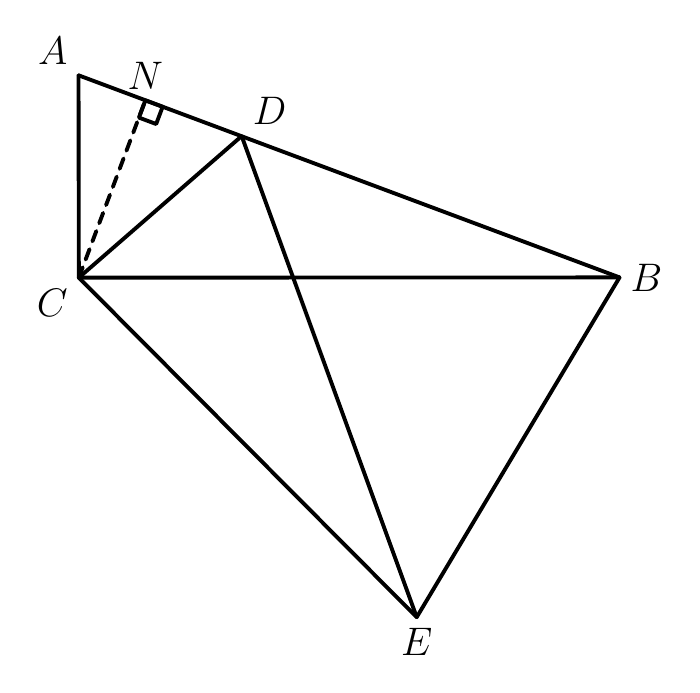
\begin{tikzpicture}[line width=1.4pt, line join=round, line cap=round]

% Named coordinates: s = 0.018223 cm/px, x = px*s, y = -py*s
\coordinate (A) at (0.984,-0.624);
\coordinate (N) at (1.833,-0.942);
\coordinate (D) at (3.056,-1.396);
\coordinate (B) at (7.855,-3.191);
\coordinate (C) at (0.988,-3.194);
\coordinate (E) at (5.279,-7.506);

% Right-angle mark corners at N (square of side about 0.23 cm)
\coordinate (m1) at (2.052,-1.024);
\coordinate (m2) at (1.970,-1.243);
\coordinate (m3) at (1.751,-1.161);

% Solid segments, all terminating exactly at vertices
\draw (A) -- (B);                 % AB through N and D
\draw (C) -- (B);                 % BC, ends at C (no left overhang)
\draw (A) -- (C);                 % CA, ends at C (no overhang below C)
\draw (D) -- (C);                 % CD, ends at C (no stub past C)
\draw (D) -- (E);                 % DE
\draw (E) -- (C);                 % EC
\draw (B) -- (E);                 % BE

% Dashed segment CN
\draw[dash pattern=on 4pt off 3pt] (C) -- (N);

% Single right-angle mark at N
\draw (N) -- (m1) -- (m2) -- (m3) -- cycle;

% Labels
\node[above left, font=\fontsize{14.5}{17.4}\selectfont] at (A) {$A$};
\node[above, font=\fontsize{14.5}{17.4}\selectfont] at (N) {$N$};
\node[above right, font=\fontsize{14.5}{17.4}\selectfont] at (D) {$D$};
\node[below left, font=\fontsize{14.5}{17.4}\selectfont] at (C) {$C$};
\node[right, font=\fontsize{14.5}{17.4}\selectfont] at (B) {$B$};
\node[below, font=\fontsize{14.5}{17.4}\selectfont] at (E) {$E$};

\end{tikzpicture}
\end{document}